
\documentclass[11pt]{article}

\usepackage{graphicx} \usepackage{float} \usepackage{epstopdf}
\usepackage{xcolor}
\usepackage{amsmath}

\renewcommand{\baselinestretch}{1.2} \setlength{\topmargin}{-0.5in}
\setlength{\textwidth}{6.5in} \setlength{\oddsidemargin}{0.0in}
\setlength{\textheight}{9.1in}

\newlength{\pagewidth} \setlength{\pagewidth}{6.5in} \pagestyle{empty}

\def\pp{\par\noindent}

\newenvironment{bsmallmatrix}
  {\left[\begin{smallmatrix}}
  {\end{smallmatrix}\right]}

\begin{document}
\centerline{\bf CSE 350 -- Theory of Computation (Honors), Spring 2018}
\medskip
\centerline{Assignment 2}
\bigskip

\bigskip
\newcounter{problemctr}

\centerline{\bf Part A}

\addtocounter{problemctr}{1}
\bigskip
\noindent
$\underline{\rm Problem\ \theproblemctr}$ \pp

\noindent
Construct a regular expression for the language of strings on
$\Sigma = \{\mbox{a}, \mbox{b}\}$
that end in ``aba'' or ``bab''.
Construct a DFA for it.\\

Regex: $\Sigma^*(aba\cup bab)$

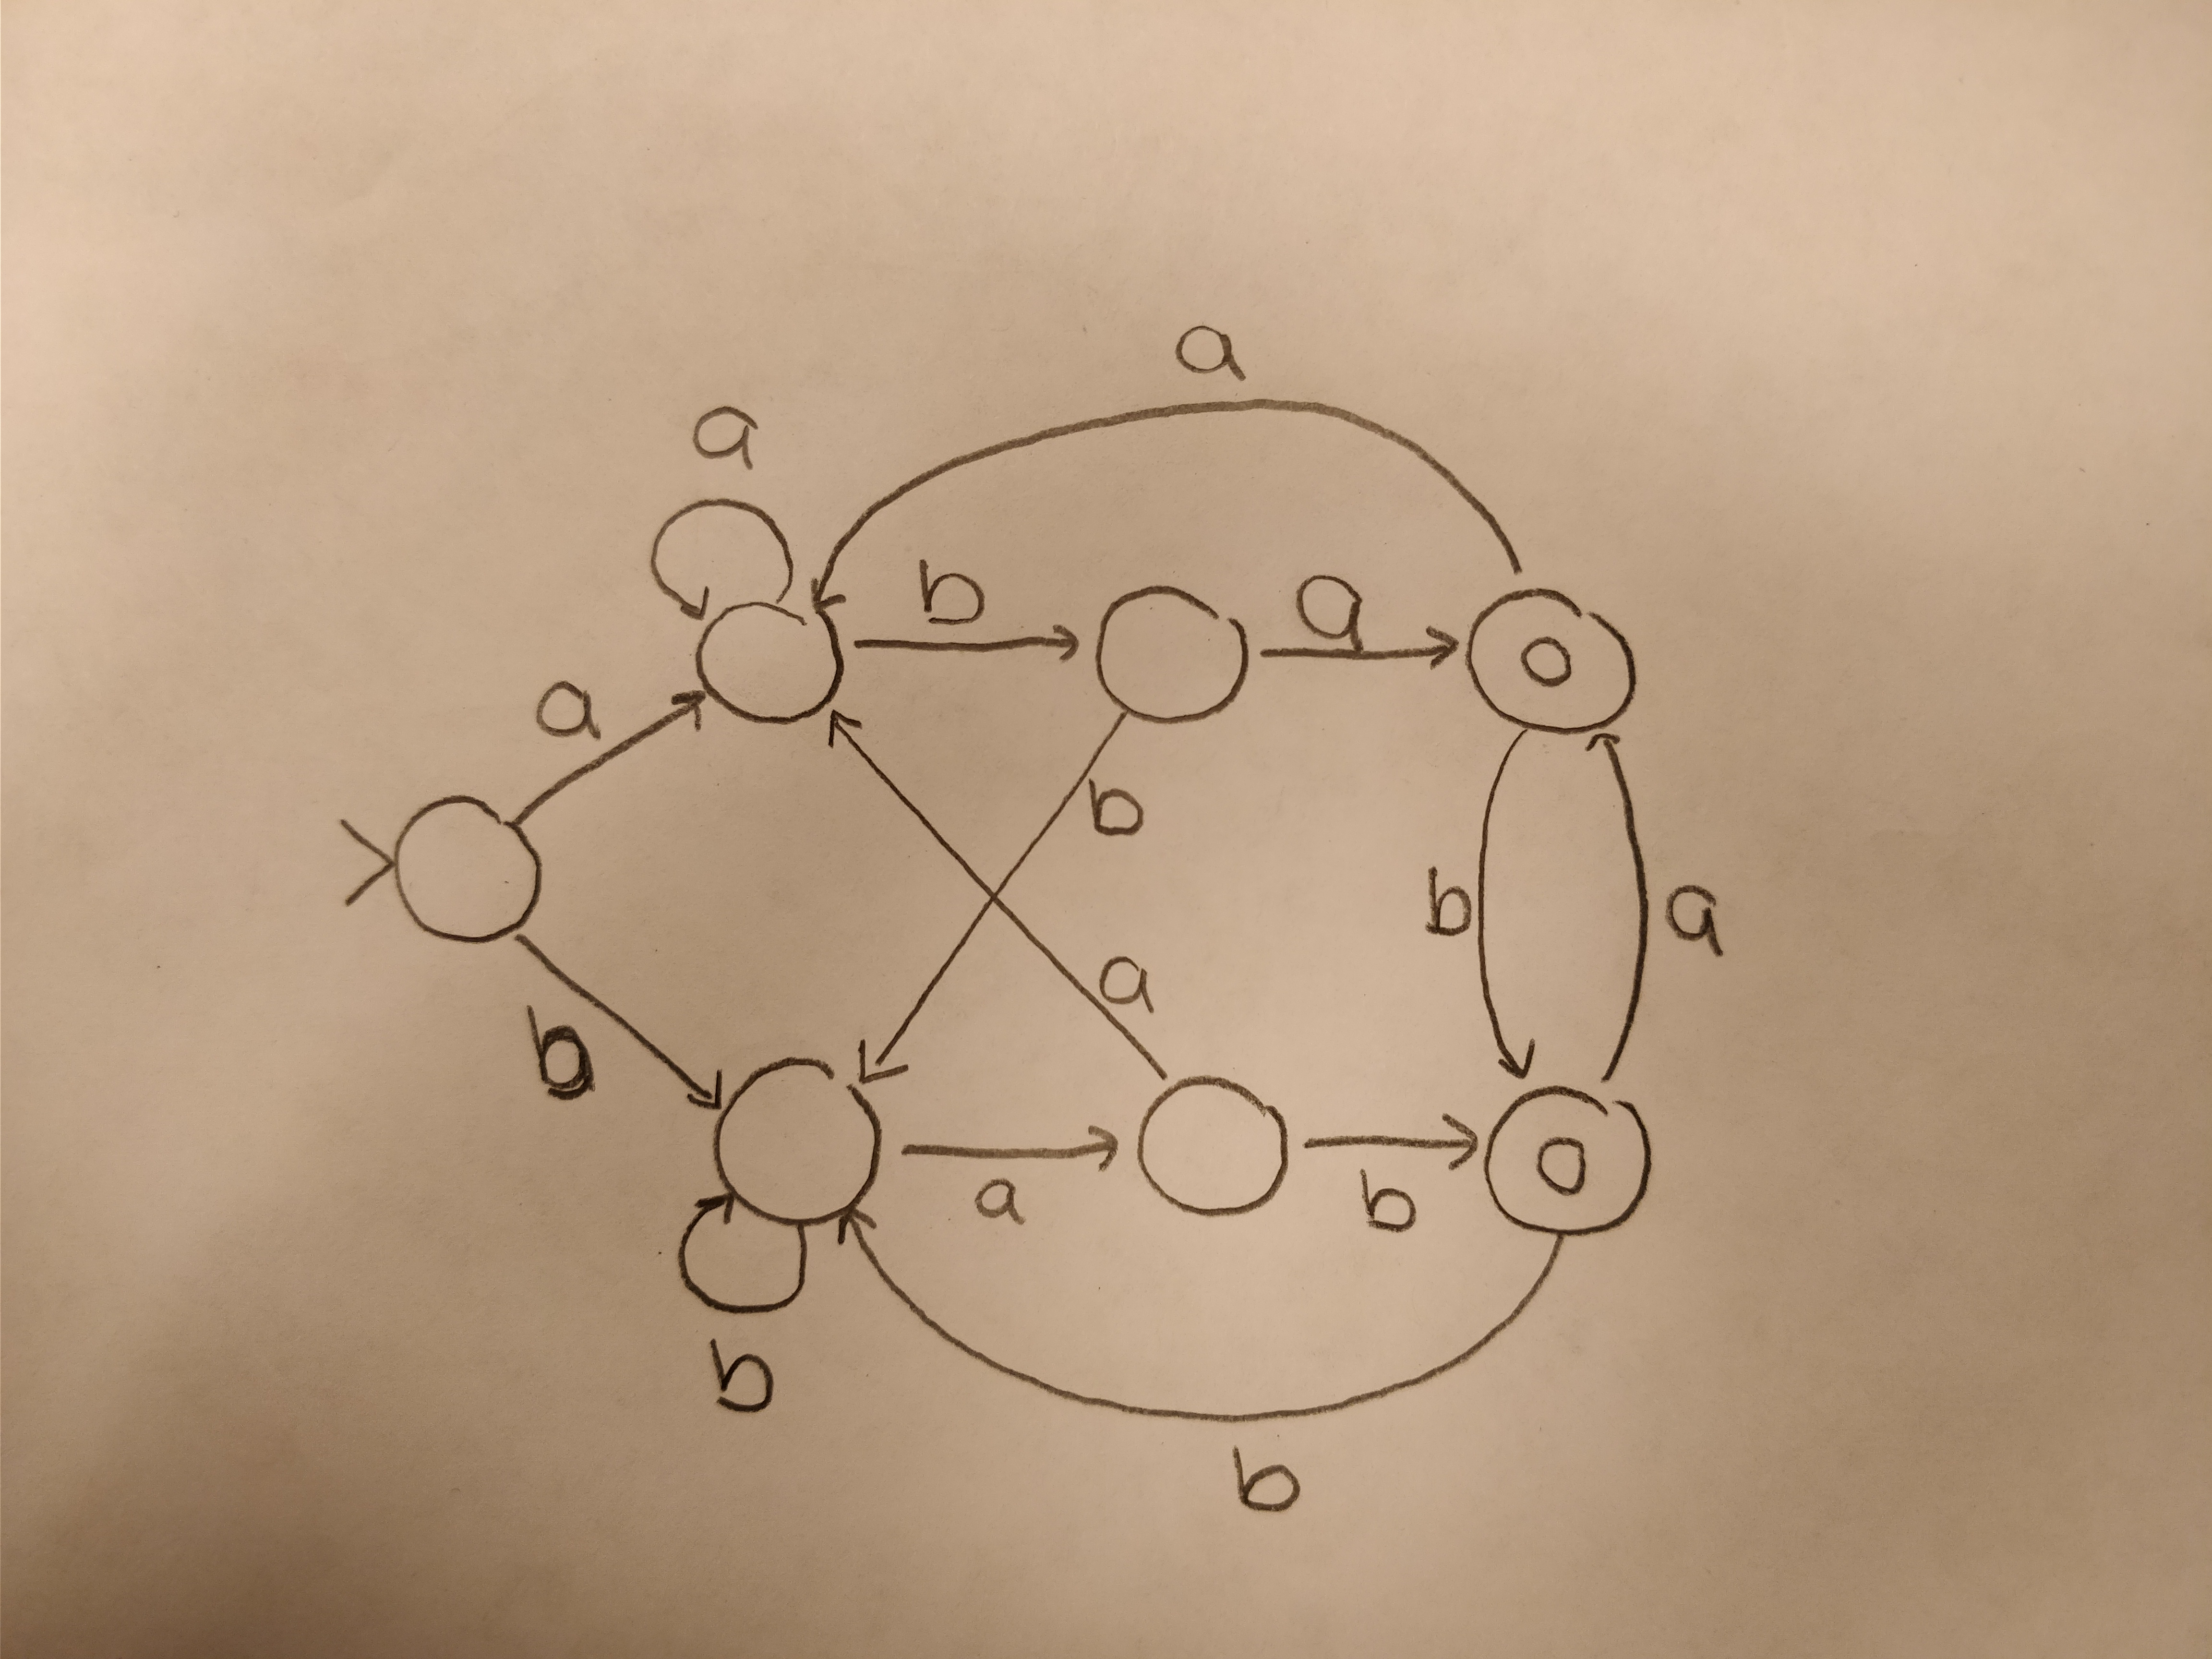
\includegraphics[scale=0.1]{q1.jpg}

\addtocounter{problemctr}{1}
\bigskip
\noindent
$\underline{\rm Problem\ \theproblemctr}$ \pp

\noindent
Let $L$ be a regular language. Can you construct an NFA for $L$ that has only one accepting state? Can you construct a DFA for $L$ that has only one accepting state? Justify.\\

We can construct an NFA for any regular language $L$ because NFAs are permitted to use empty string transitions between nodes. If the regular language has a form where there are multiple accepting states, all but one accepting states can be removed and instead an empty string can lead to the remaining accepting state.\\

We cannot construct a DFA for all regular languages. A simple counterexample would be the language containing the empty string or an odd number of $a$s. The regular expression would be $e\cup a(aa)*$\\

\addtocounter{problemctr}{1}
\bigskip
\noindent
$\underline{\rm Problem\ \theproblemctr}$ \pp

\noindent
For any string $w = w_1 w_2 \cdots w_n$, where each $w_i$ is a character, the reverse of $w$, written $w^R$, is the string $w$ in reverse order, $w_n \cdots w_2 w_1$. For any language $A$, let $A^R = \{w^R | w \in A\}$. Show that if $A$ is regular, so is $A^R$.\\

If $A$ is of the form $(k, \Sigma, s, \delta, F)$, the DFA $A_R$ would be of the form $(k, \Sigma, s_R, \delta_R, F_R)$.\\

$s_R$ is a state that combines all the accepting states in F.\\
$F_R=s$\\
$\delta_R=\{((x,z),y)|\forall((y,z),x)\in\delta \land x,y\neq s\}\cup \{((s_R, z), x)|\forall((x,z),y)\in \delta, y\in F\}\cup \{((y, z), s_R)|\forall((x,z),y)\in \delta, x\in F\}$\\

Essentially the DFA where the accepting and starting states have been switched and transitions have reversed directions.\\

\addtocounter{problemctr}{1}
\bigskip
\noindent
$\underline{\rm Problem\ \theproblemctr}$ \pp

\noindent
Let

\begin{equation*}
  \Sigma_3 =
  \left \{
  \begin{bsmallmatrix}0 \\ 0 \\ 0\end{bsmallmatrix},
  \begin{bsmallmatrix}0 \\ 0 \\ 1\end{bsmallmatrix},
  \begin{bsmallmatrix}0 \\ 1 \\ 0\end{bsmallmatrix},
  ...
  \begin{bsmallmatrix}1 \\ 1 \\ 1\end{bsmallmatrix}
  \right \}.
\end{equation*}

$\Sigma_3$ contains all size 3 columns of 0s and 1s. A string of symbols in
$\Sigma_3$ gives 3 rows of 0s and 1s. Consider each row to be a binary number
and let

\begin{equation*}
  B = \{ w \in \Sigma_3^*\, |\, \mbox{the bottom row of } w \mbox{ is the sum of the top two rows} \}.
\end{equation*}

For example,

\begin{equation*}
  \begin{bsmallmatrix}0\\0\\1\end{bsmallmatrix}
  \begin{bsmallmatrix}1\\0\\0\end{bsmallmatrix}
  \begin{bsmallmatrix}1\\1\\0\end{bsmallmatrix}
  \in B,
  \mbox{ but }
  \begin{bsmallmatrix}0\\0\\1\end{bsmallmatrix}
  \begin{bsmallmatrix}1\\0\\1\end{bsmallmatrix}
  \not \in B.
\end{equation*}

Show that $B$ is regular. (Hint: Working with $B^R$ is easier. You may assume
the result proven in problem 3.)

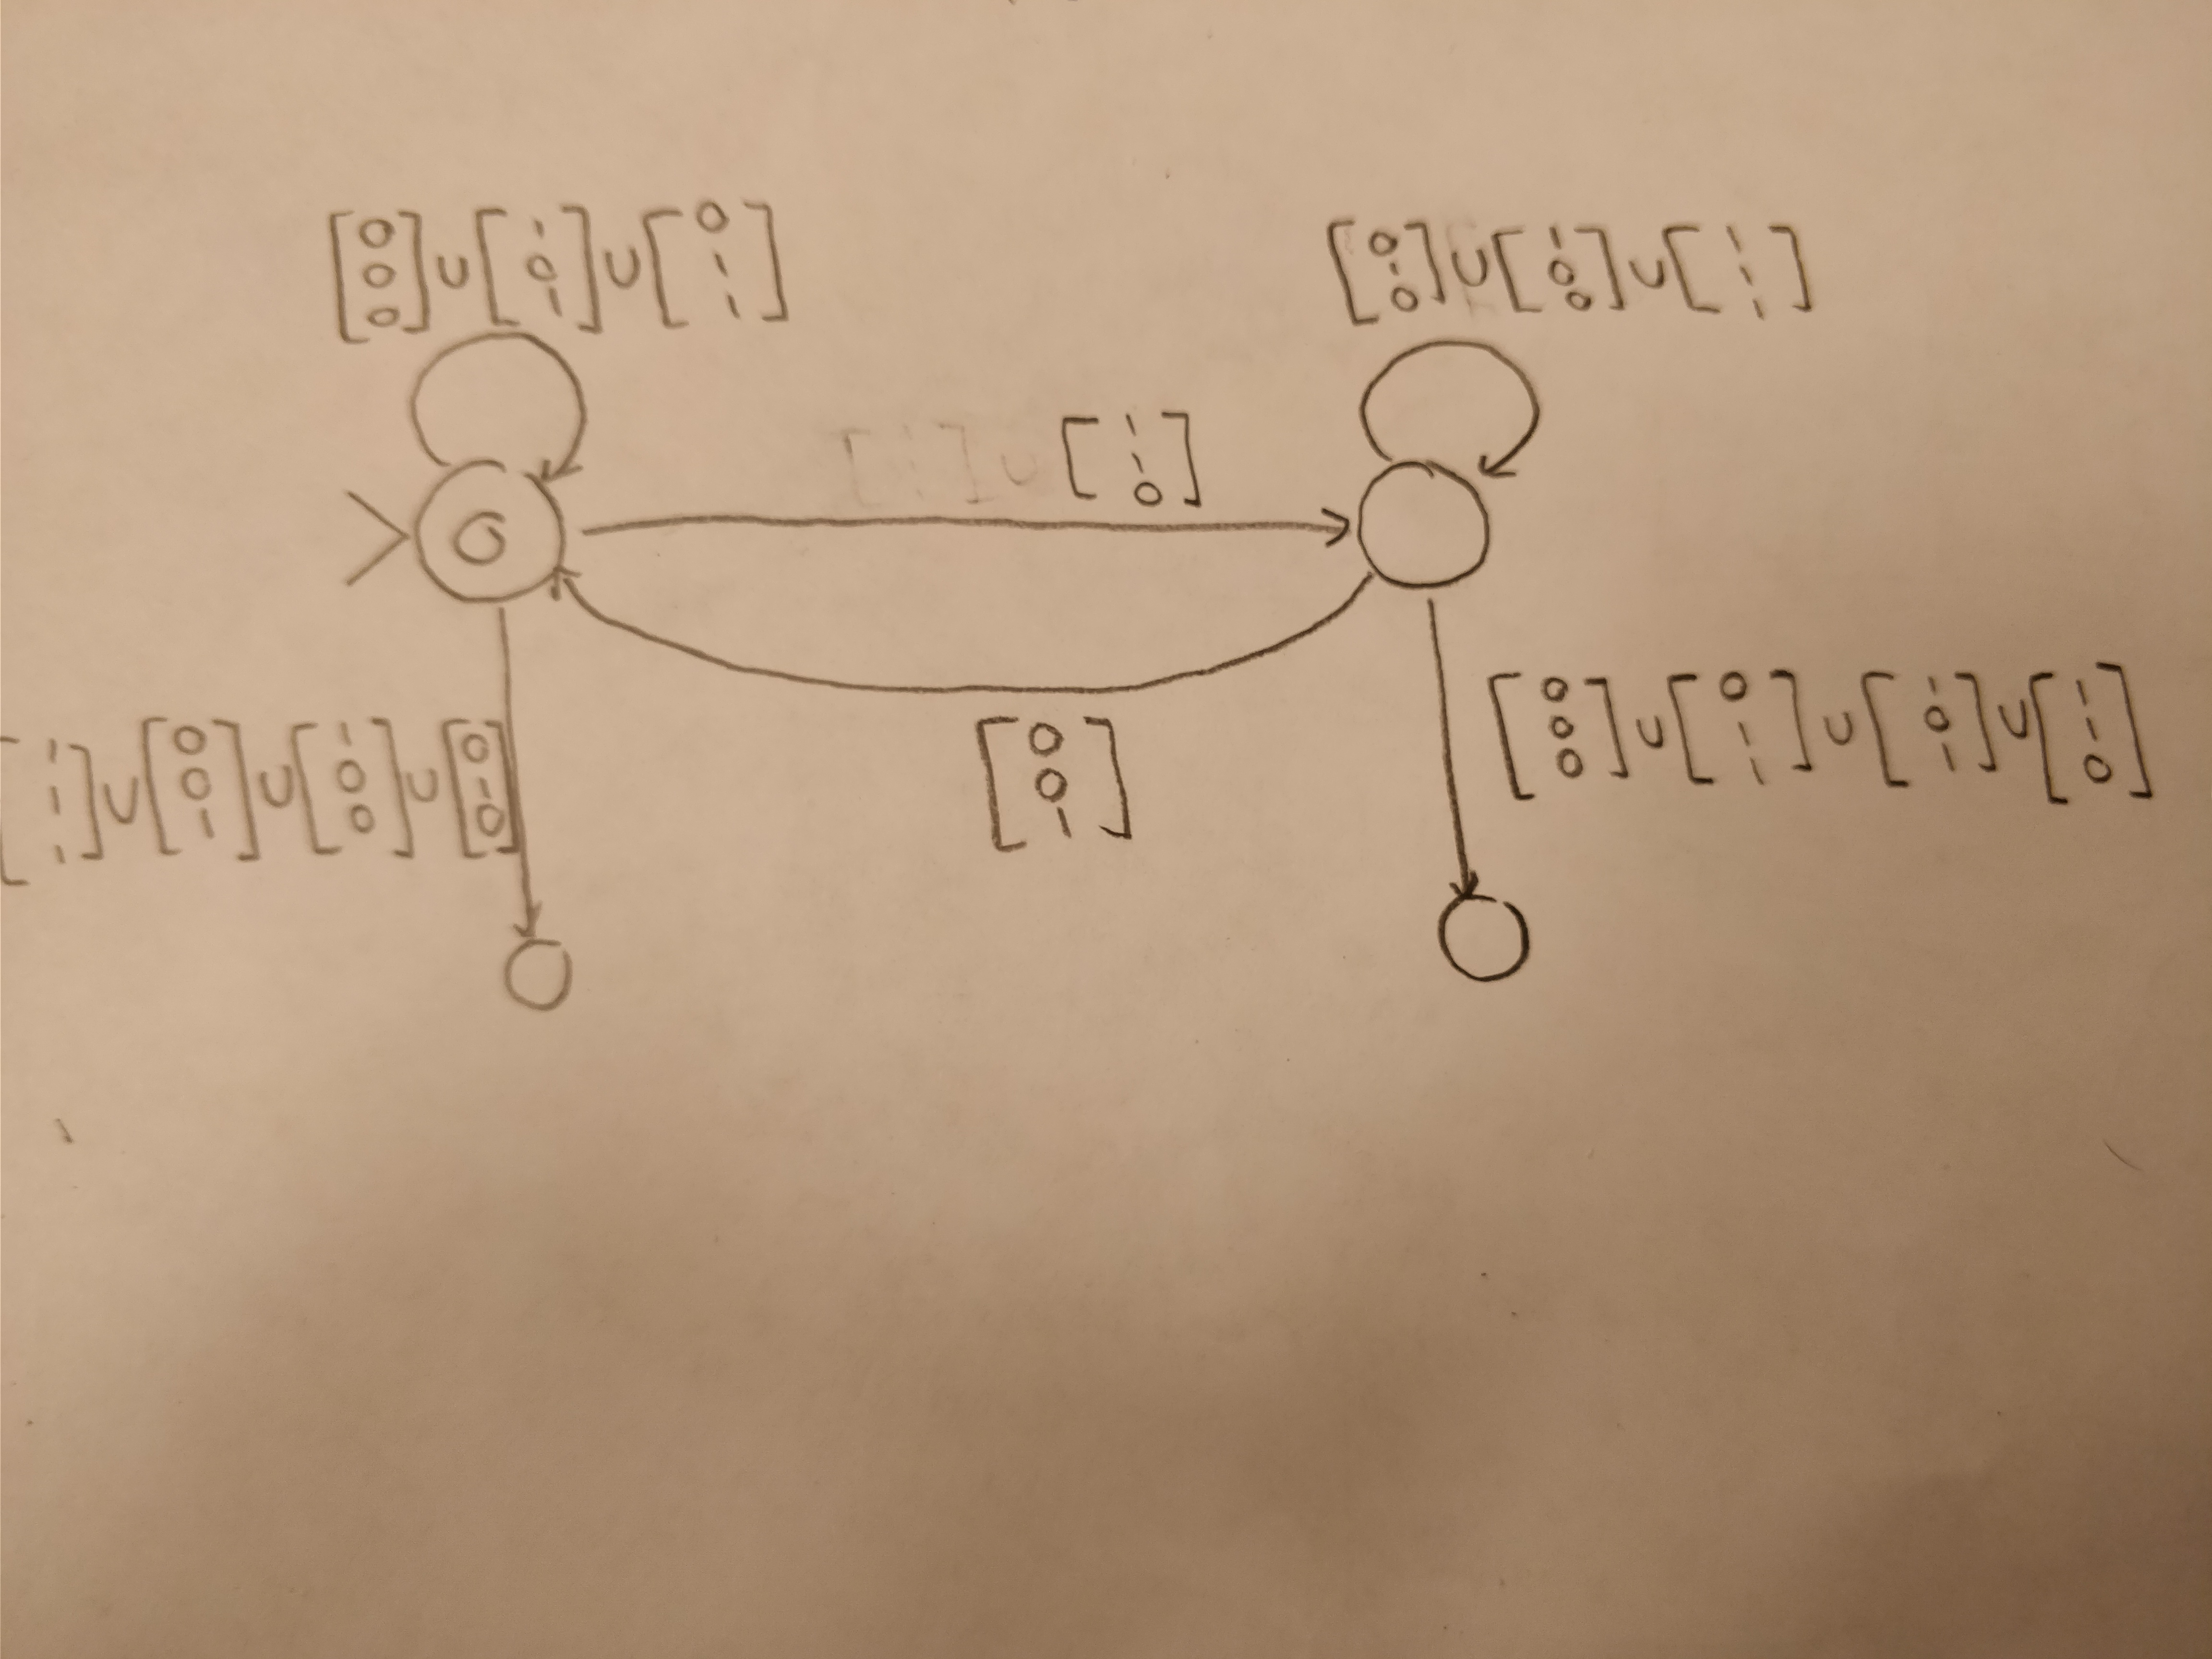
\includegraphics[scale=0.1]{q4.jpg}

Above is the DFA for $B^R$, which means that $B$ is also regular.

* Credit to Andy Liang for correcting an issue with the DFA

\end{document}